\chapter{Analysis and specification of requirements}
\newpage

\setcounter{secnumdepth}{0} % Set the section counter to 0 so next section is not counted in toc
% ----------------------- Introduction ----------------------- %
\section{Introduction}
In this chapter, we are going to analyze the specification and the requirements of the application, mostly this chapter will contains the product main features and their conception so we will have our expectation for the end result.
\setcounter{secnumdepth}{3} % Resume counting the sections for the toc with a depth of 2 (Sections and sub-sections)

% ----------------------- Requirements ----------------------- %
\section{Requirements}
Our requirements are divided into two parts, the clients portal of the application called Dashboard, and the lead generating and handling happening in the background.
\subsection{Dashboard}
\subsubsection{Requirements}
Here is a global use case diagram that specifies the dashboard requirements :
\makebox[\textwidth]{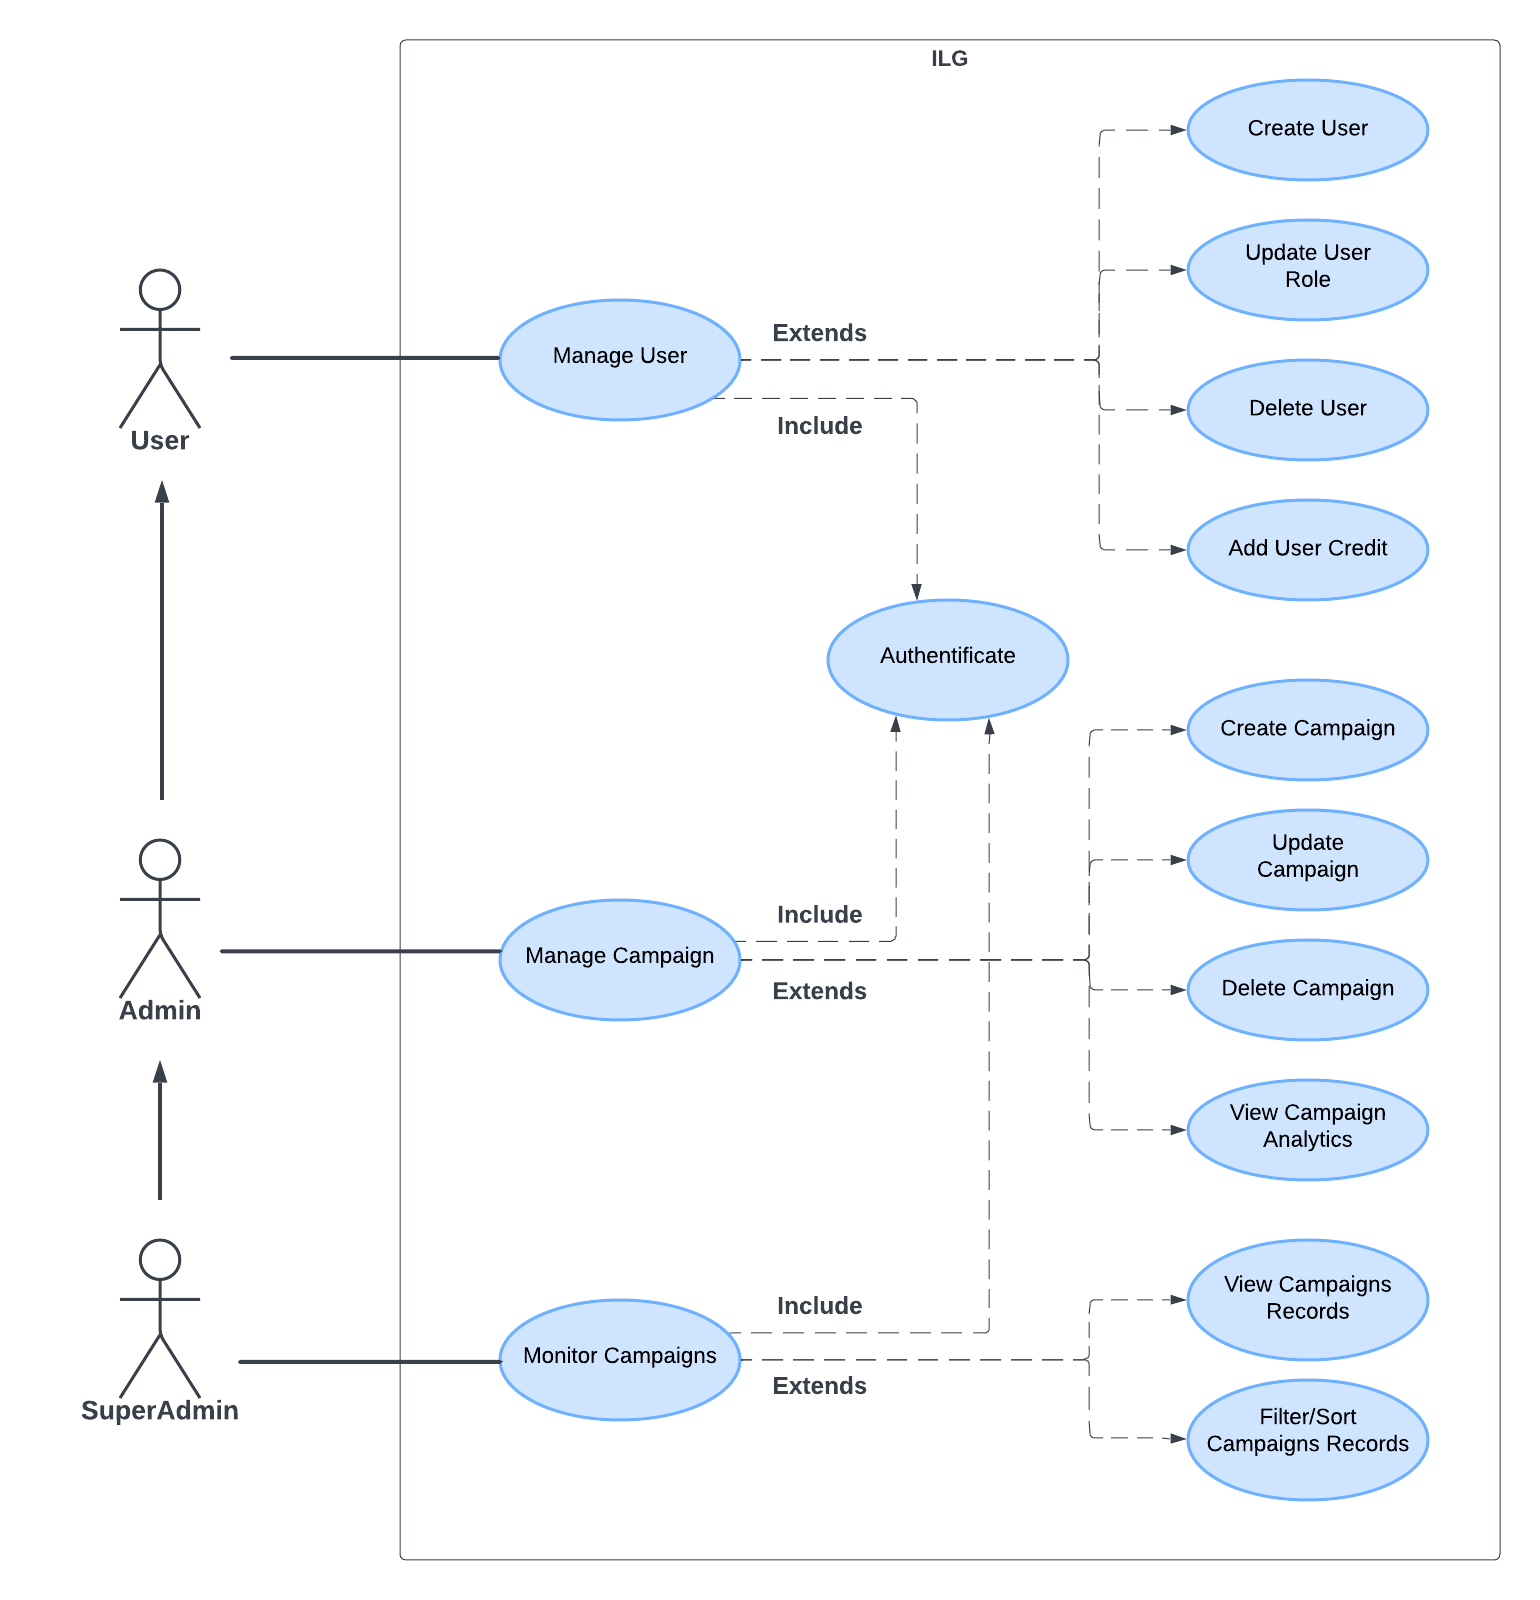
\includegraphics[width=15cm]{src/assets/diagrams/usecase.png}}
\subsubsection{User management}
\subsubsection{Campaign management}
\subsubsection{Campaign monitoring}
% TODO : CHANGE_ME
\subsection{Lead generating}
\subsubsection{Requirements}
\subsubsection{Scraping leads}
\subsubsection{Contacting Leads}

% TODO : CHANGE_ME
\newpage
\section{Conception}
In this section, we will dive deep into the conception and the logic behind the parts of the application :
\subsection{Architecture}
\subsubsection{Microservices}
\begin{table}[H]
	\renewcommand{\arraystretch}{1.5}%
	\caption{All the application's Microservices}
	\centering
	\medskip
	\begin{tabularx}{1\textwidth} {
			| >{\hsize=.75\hsize\linewidth=\hsize\raggedright\arraybackslash}X
			| >{\hsize=1.8\hsize\linewidth=\hsize\raggedright\arraybackslash}X
			| >{\hsize=0.45\hsize\linewidth=\hsize\raggedright\arraybackslash}X |}
		\hline
		\rowcolor{primary} \textbf {Name} & \textbf {Description}                                                                                  & \textbf {Scalable} \\
		\hline
		\textbf {ilg-data}                & GraphQL Database access layer used to feed all needed data for other services from the Postgres DB.    & No                 \\
		\hline
		\textbf {ilg-api}                 & RESTful api to serve data to the React app dashboard.                                                  & No                 \\
		\hline
		\textbf {ilg-front}               & a React app dashboard application served throw NGINX.                                                  & No                 \\
		\hline
		\textbf {ilg-scheduler}           & Service thats responsible for scheduling and orchestrating the tasks queues and notifications.         & No                 \\
		\hline
		\textbf {ilg-scraper}             & Service thats responsible for scraping leads of campaigns links from LinkedIn Sales Navigator.         & Yes                \\
		\hline
		\textbf {ilg-automation}          & Service thats responsible for handling LinkedIn accounts inboxs/threads and sendings invites to leads. & Yes                \\
		\hline
	\end{tabularx}
\end{table}
\newpage
\subsubsection{Cloud Infrastructure}
Since we are using a Kubernetes Cluster for our Cloud Infrastructure, we decided to distribute our different microservices into their corresponding nodes (VMs) depending on their shared components and scalabity. So here is an overview of the current Cloud Infrastructure of the application :
\linebreak
\makebox[\textwidth]{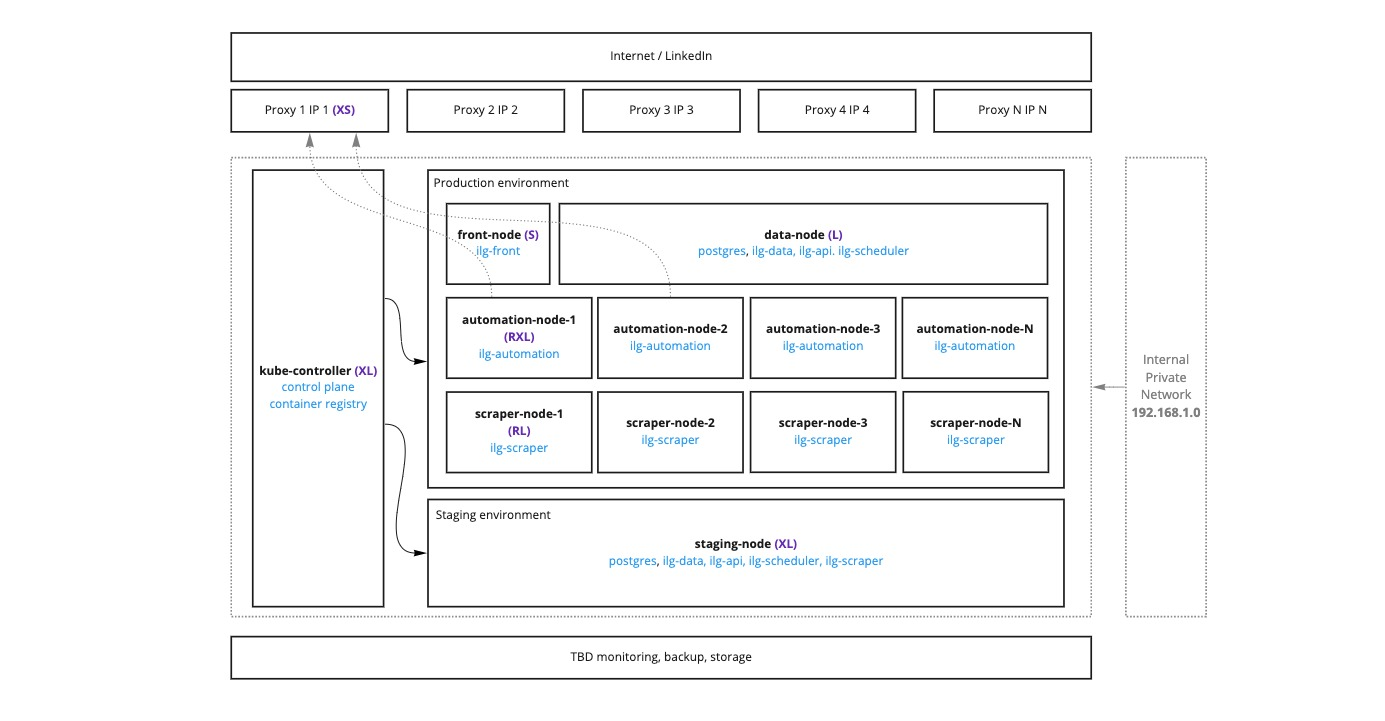
\includegraphics[width=24cm]{src/assets/diagrams/cloud_infra.jpeg}}
\subsection{Dashboard}
\subsubsection{Conception of the features}
\newpage
\subsection{Tasks \& Queues}
\subsubsection{Thoery of tasks and queues}
Task queues let applications perform work, called tasks, asynchronously outside of a user request. If an app needs to execute work in the background, it adds tasks to task queues. The tasks are executed later, by worker services. The Task Queue service is designed for asynchronous work.
\linebreak
\makebox[\textwidth]{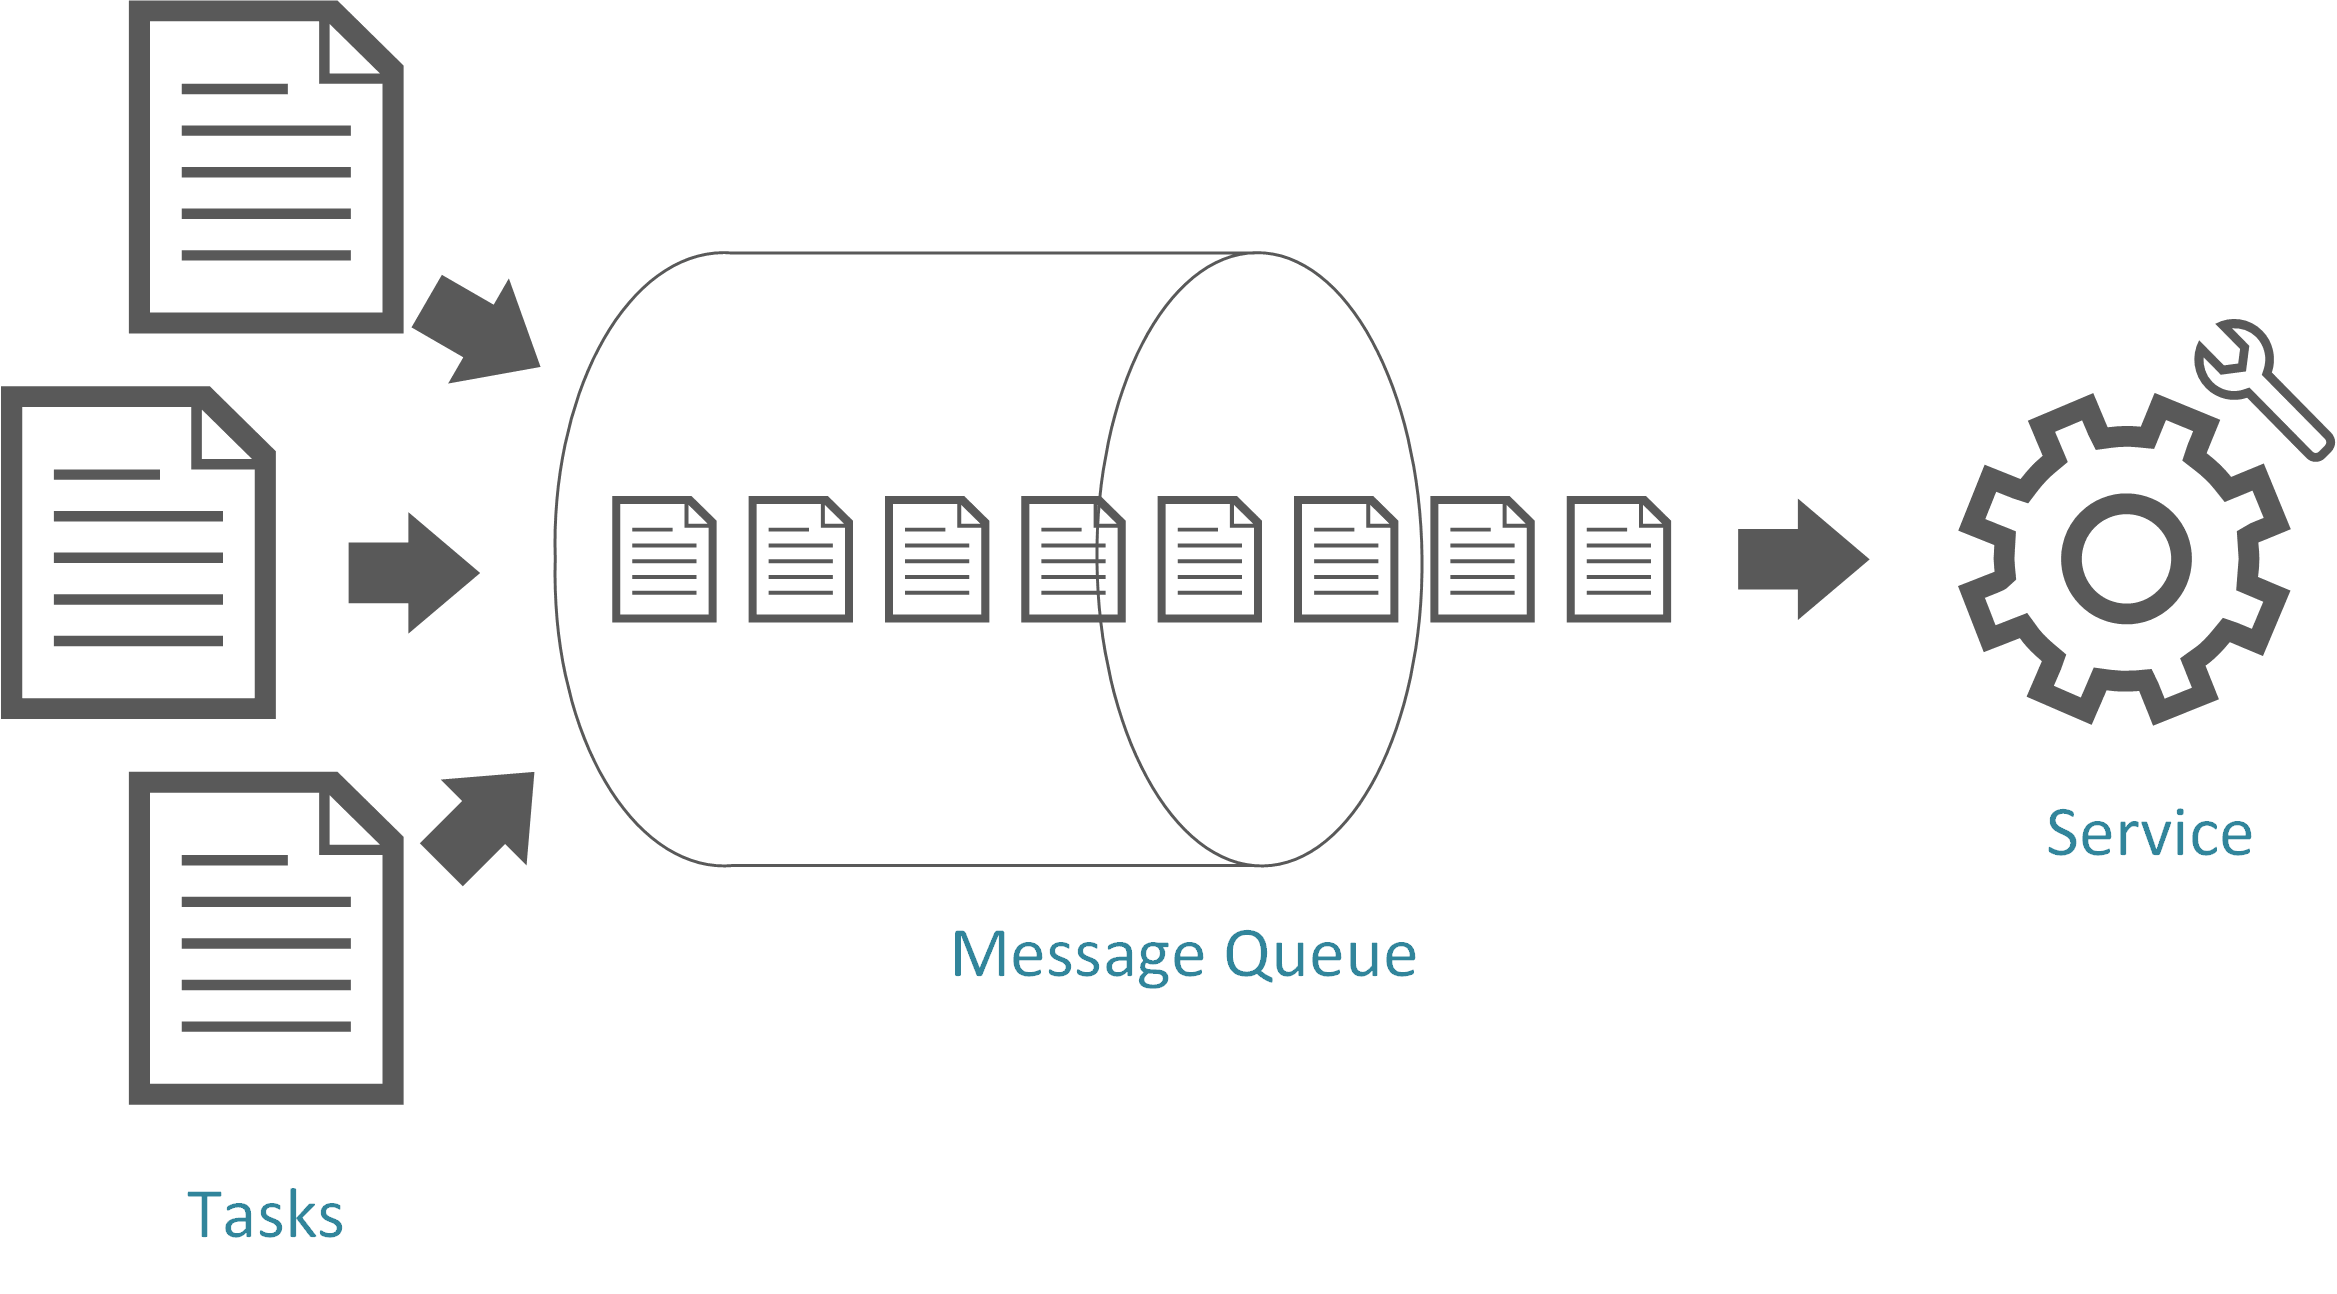
\includegraphics[width=12cm]{src/assets/diagrams/task-queue.png}}
\subsubsection{Tasks queues types}
\begin{table}[H]
	\renewcommand{\arraystretch}{1.5}%
	\caption{All the application's tasks/jobs}
	\centering
	\medskip
	\begin{tabularx}{1\textwidth} {
			| >{\hsize=1.2\hsize\linewidth=\hsize\raggedright\arraybackslash}X
			| >{\hsize=1.2\hsize\linewidth=\hsize\raggedright\arraybackslash}X
			| >{\hsize=0.8\hsize\linewidth=\hsize\raggedright\arraybackslash}X
			| >{\hsize=0.8\hsize\linewidth=\hsize\raggedright\arraybackslash}X |}
		\hline
		\rowcolor{primary} \textbf {Name} & \textbf {Description}                                             & \textbf {Producer} & \textbf {Consumer} \\
		\hline
		\textbf {campaign-scrape}         & Scrape list of leads from campaign search list                    & ilg-scheduler      & ilg-scraper        \\
		\hline
		\textbf {lead-scrape}             & Scrape lead information and save them in the database             & ilg-scraper        & ilg-scraper        \\
		\hline
		\textbf {handle-inbox}            & Hanle conversation threads of leads and send follow ups if needed & ilg-scheduler      & ilg-automation     \\
		\hline
		\textbf {send-invite}             & Send connection invite to leads                                   & ilg-scheduler      & ilg-automation     \\
		\hline
	\end{tabularx}
\end{table}
\subsubsection{Scheduling tasks}
\makebox[\textwidth]{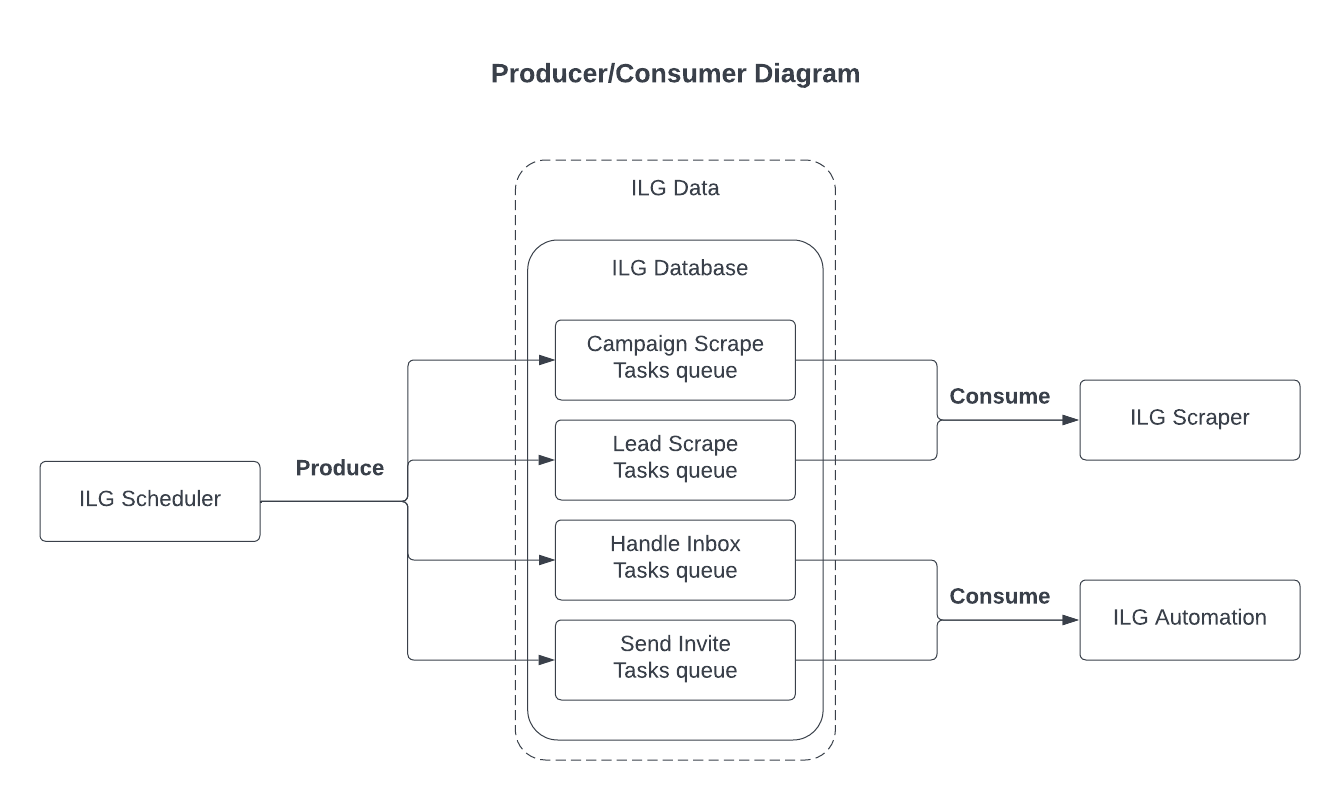
\includegraphics[width=16cm]{src/assets/diagrams/producer_consumer.png}}
\subsection{Automation \& Scraper}
\subsubsection{Automation flow}
\makebox[\textwidth]{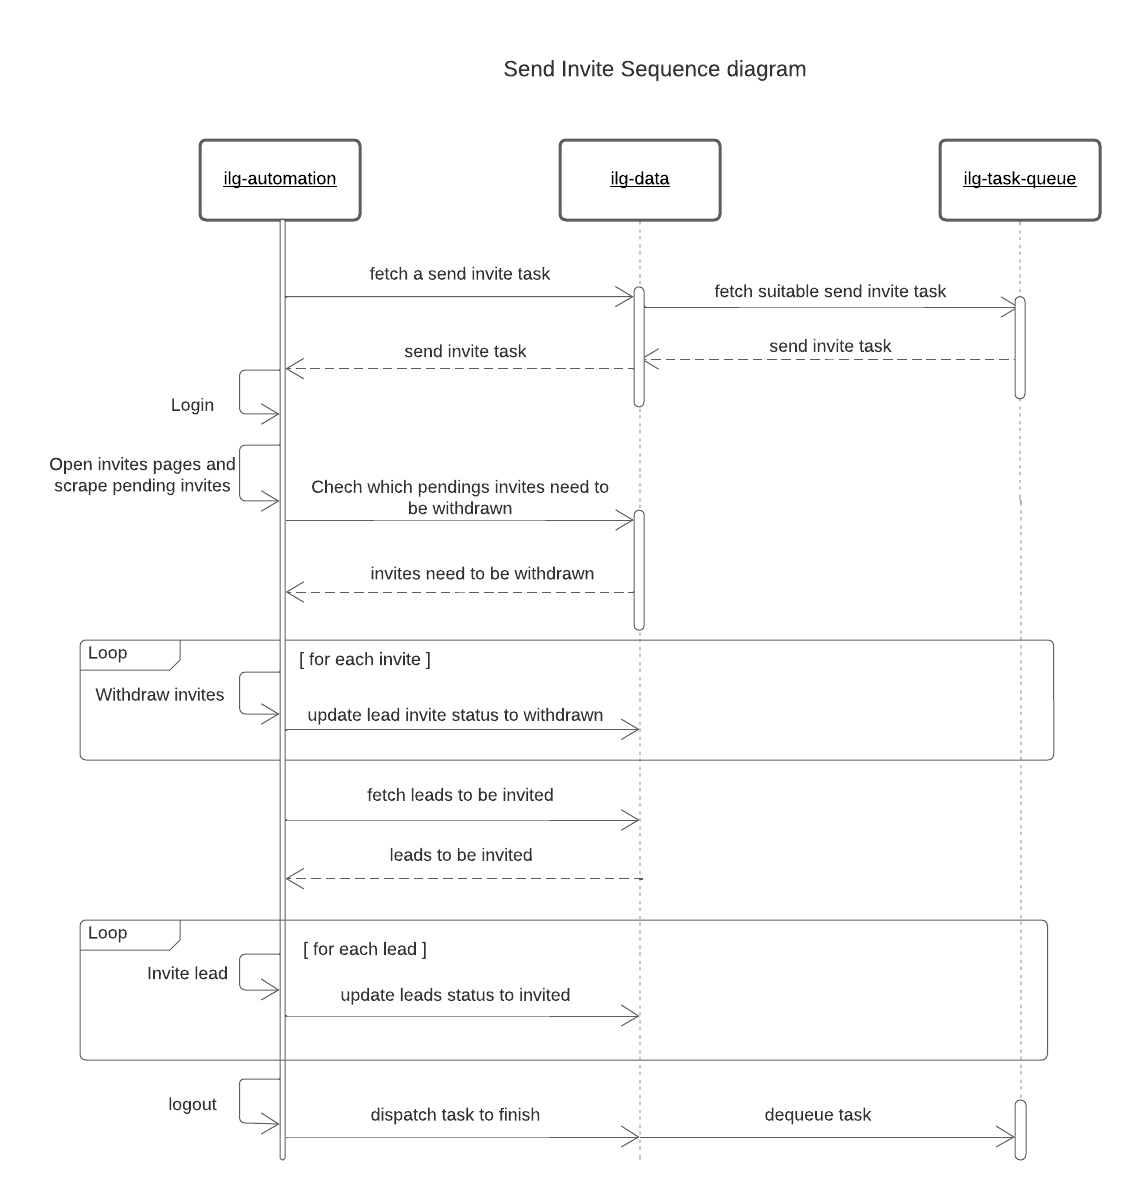
\includegraphics[width=16cm]{src/assets/diagrams/send_invite_sequence.png}}
\newpage
\makebox[\textwidth]{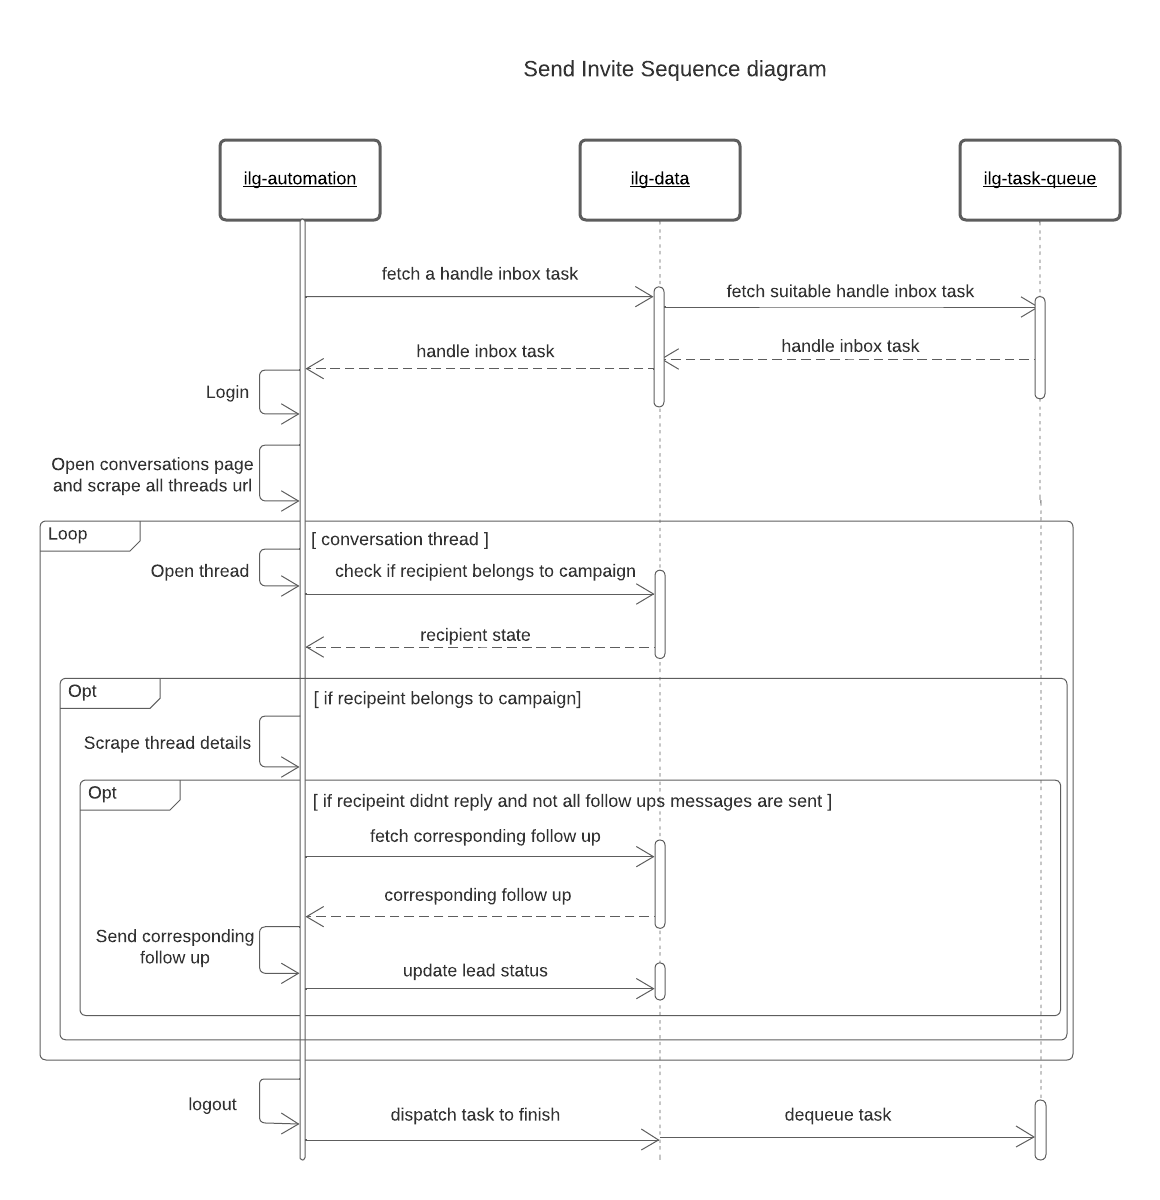
\includegraphics[width=16cm]{src/assets/diagrams/handle_inbox_sequence.png}}
\subsubsection{Scraper flow}
\makebox[\textwidth]{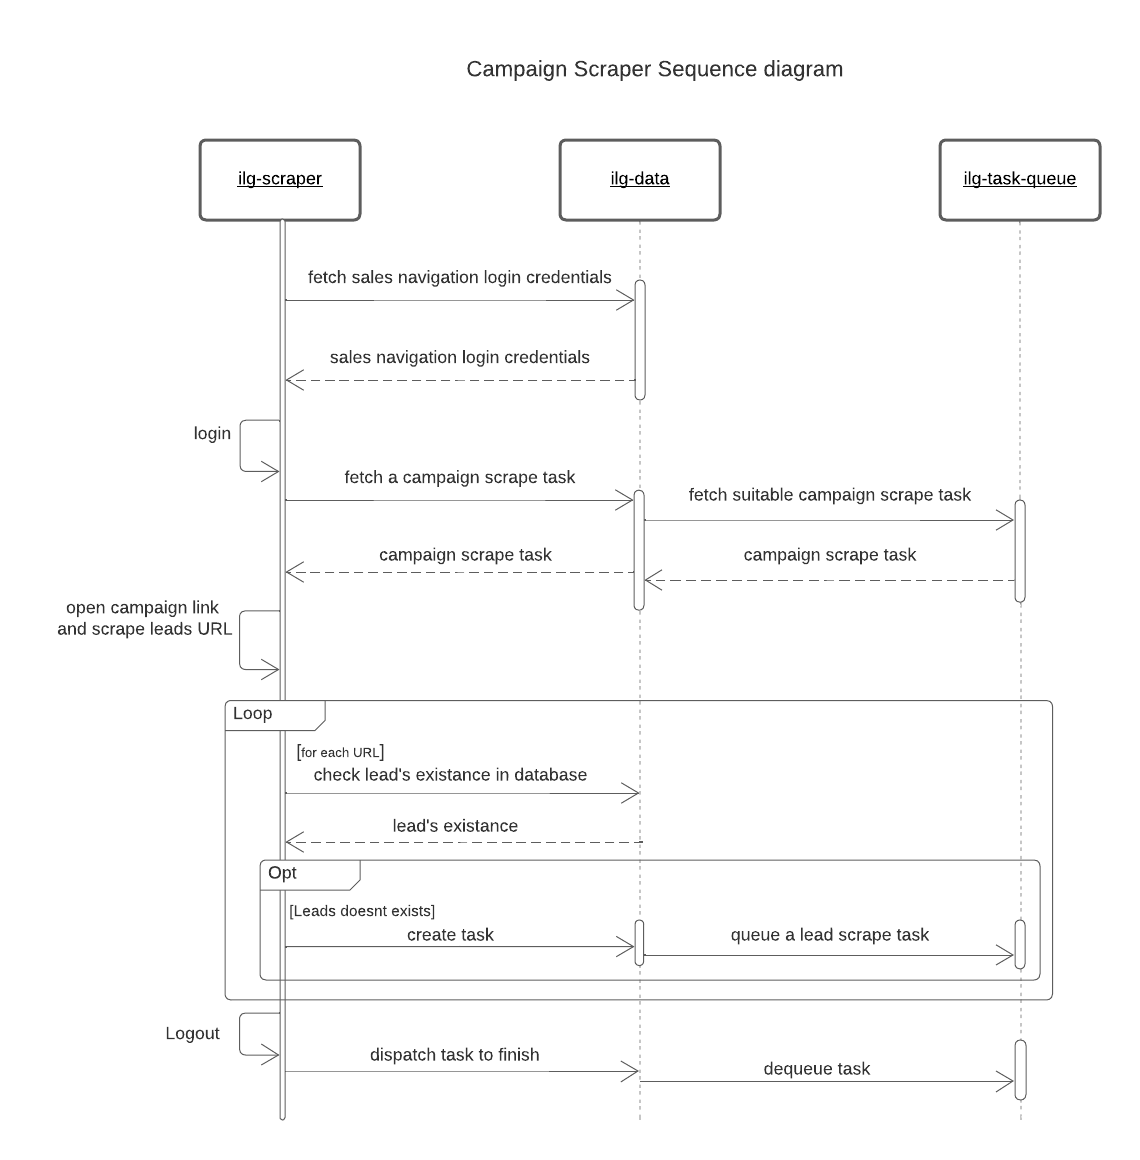
\includegraphics[width=16cm]{src/assets/diagrams/campaign_scraper_sequence.png}}
\newpage
\makebox[\textwidth]{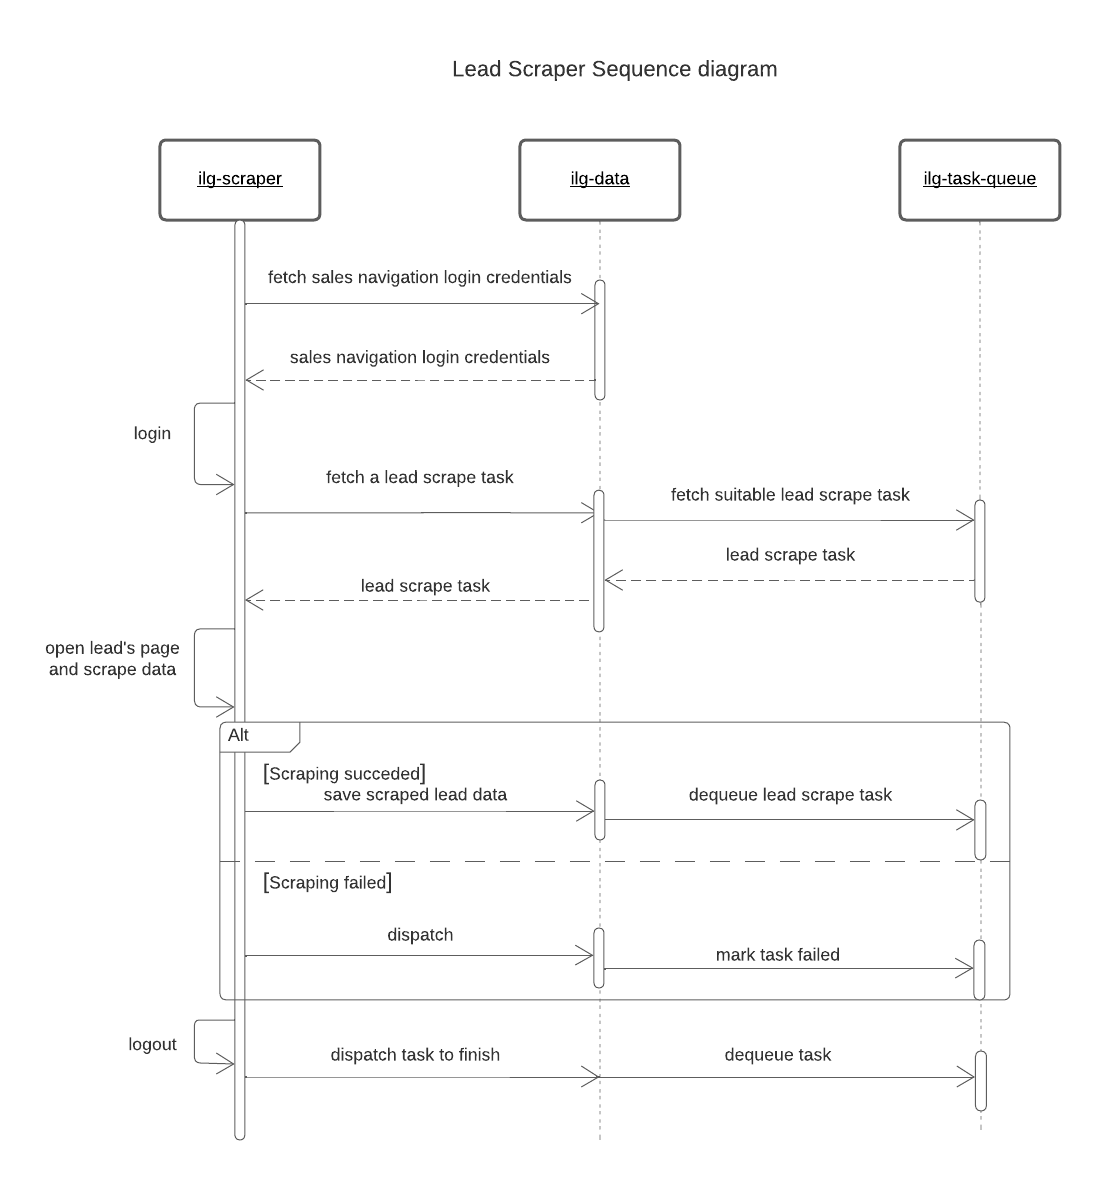
\includegraphics[width=16cm]{src/assets/diagrams/lead_scraper_sequence.png}}
\subsubsection{Horizontally Scaling}
\newpage
\subsection{Data Layer API}
\subsubsection{Schema}
\makebox[\textwidth]{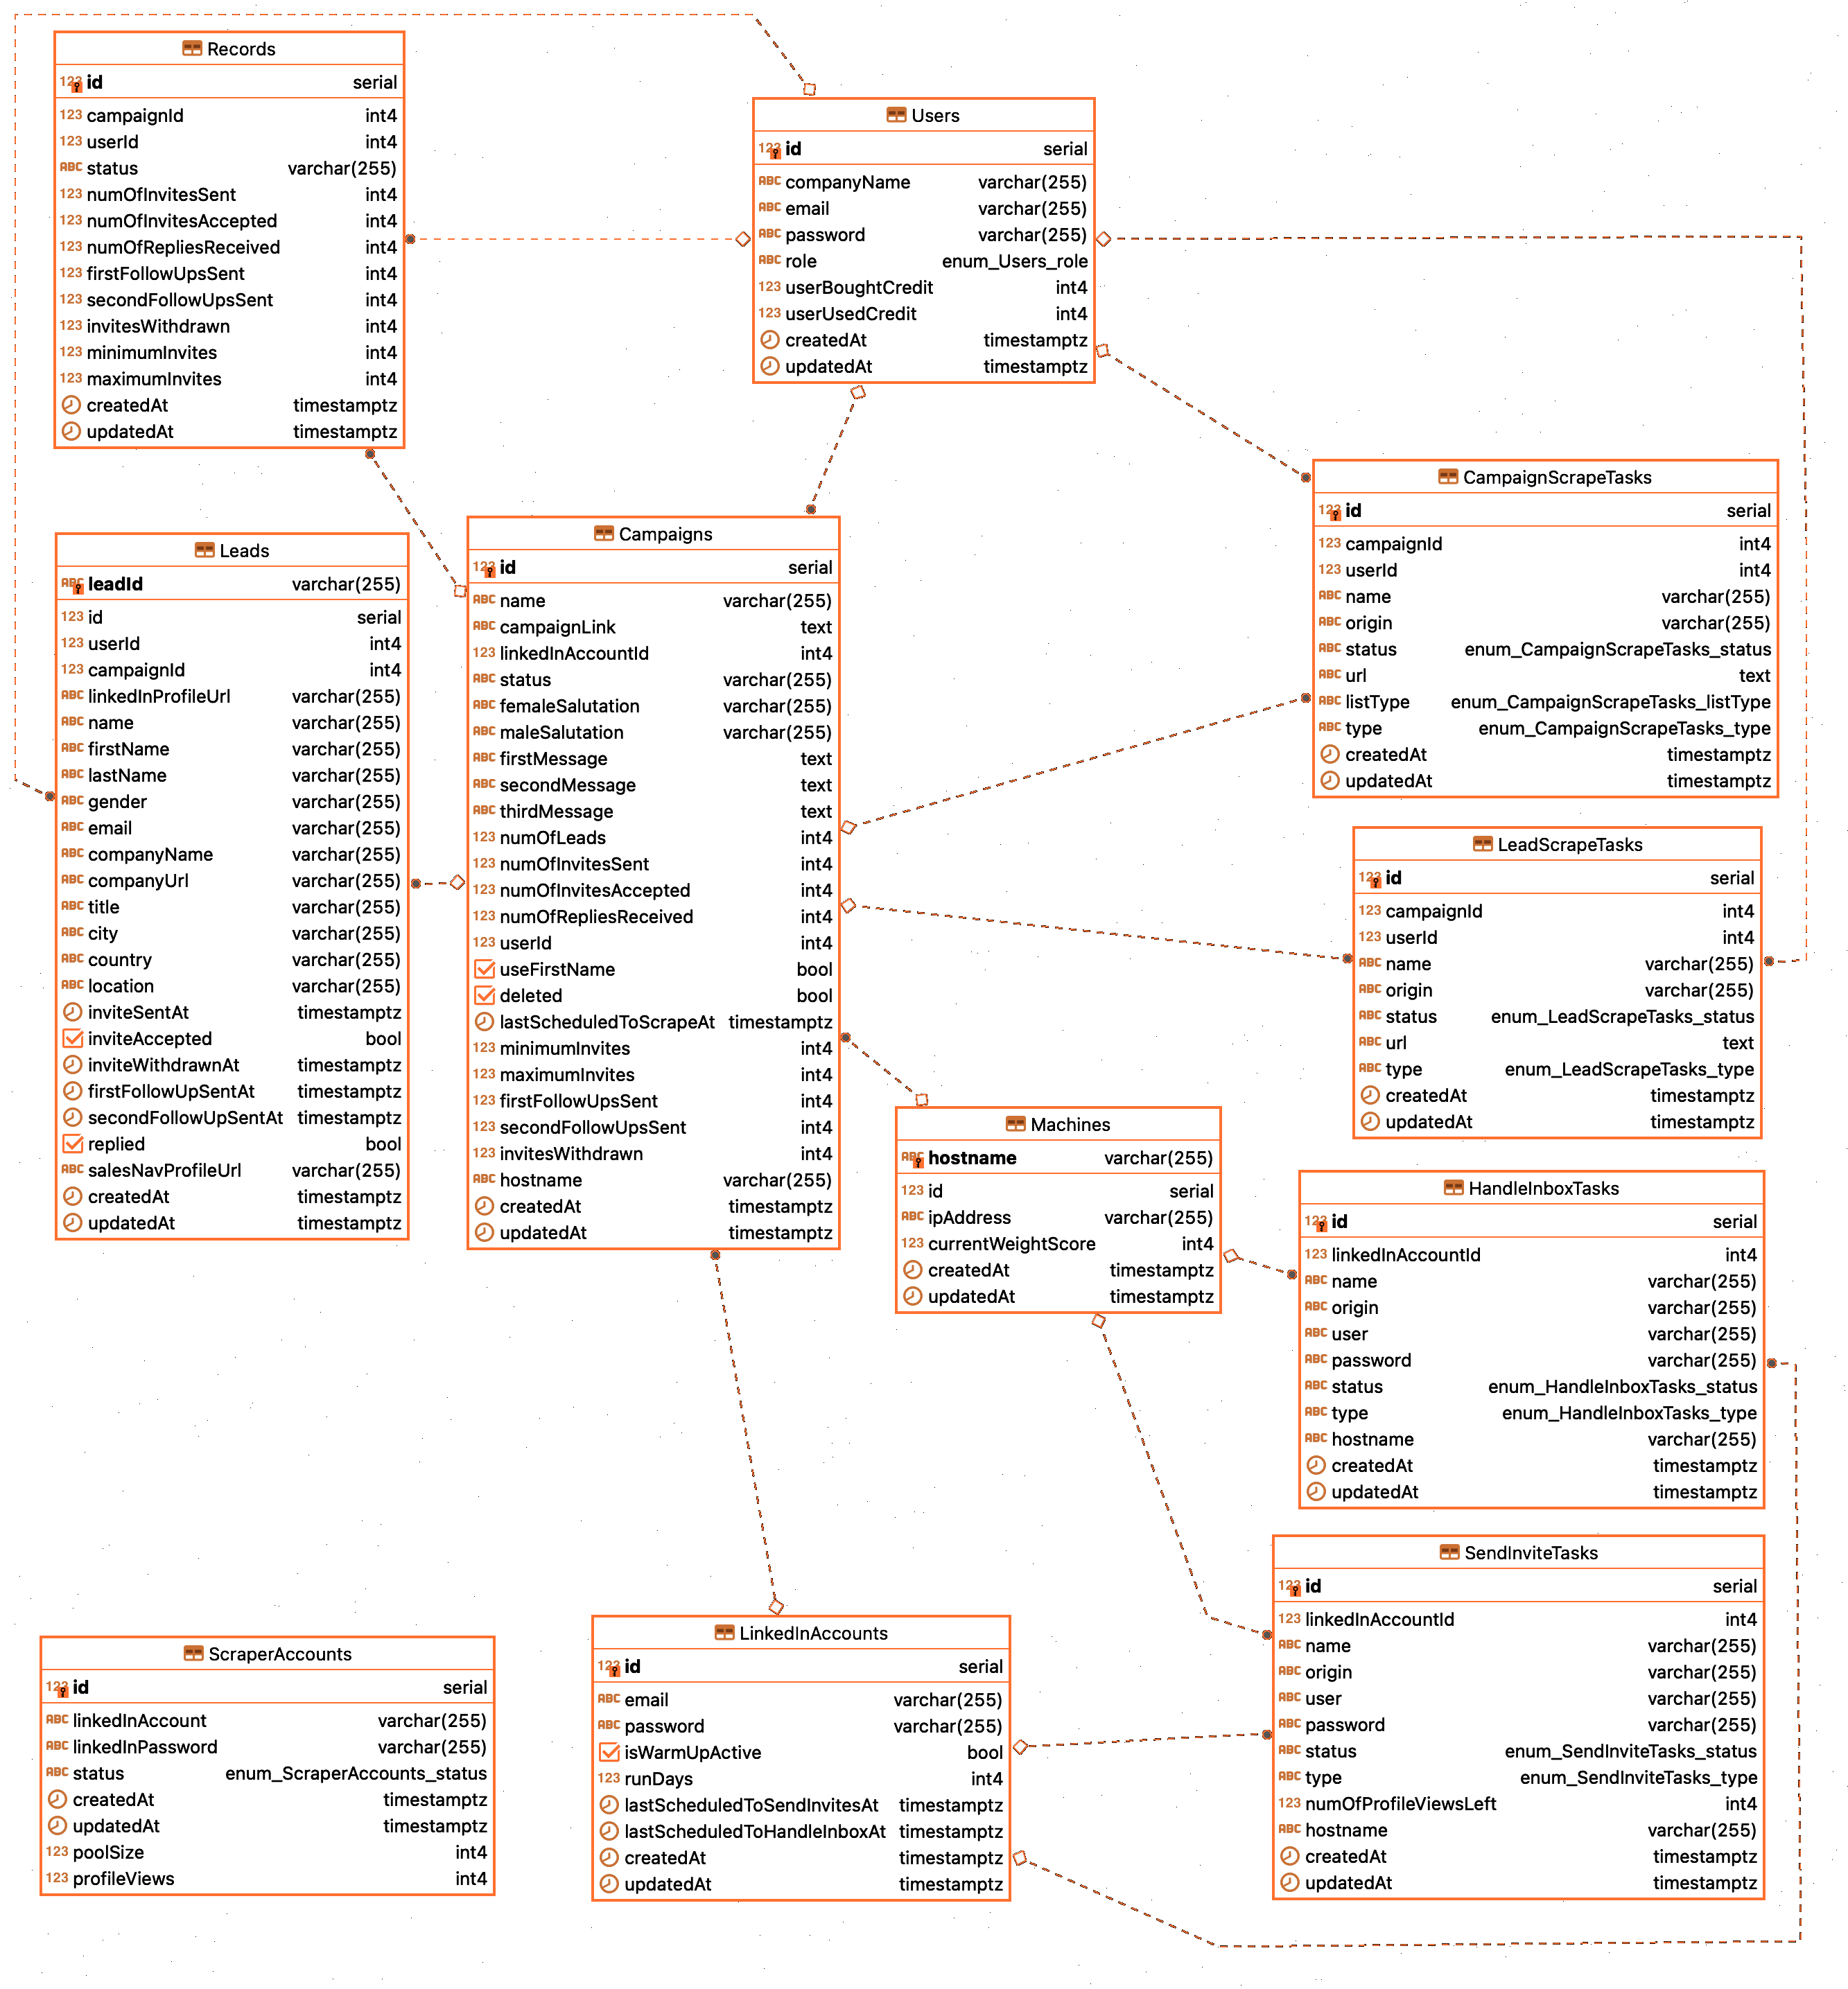
\includegraphics[width=16cm]{src/assets/diagrams/er.png}}
\subsubsection{Different interfaces}
REST and GraphQL
\newpage
\setcounter{secnumdepth}{0} % Set the section counter to 0 so next section is not counted in toc
% ----------------------- Conclusion ----------------------- %
\section{Conclusion}
\lipsum[2]
